\chapter{Less Can Be More: Pruning Street Networks for Sustainable City-Making\textsuperscript{*}}
\chaptermark{Less Can Be More: Pruning Street Nets for Sustainable City-Making}
\label{ch:less_can_be_more}
\graphicspath{{chapters/03_less_can_be_more/figures/}}

\footnotetext{* A version of this chapter has been published as a peer-reviewed article: \fullcite{ArgotaSanchez-Vaquerizo2023LessCity-making}.}


\section*{}
\chapterabstract{
Current trends in urban planning aim at the reduction of space for private vehicles to promote alternative mobility, more diverse activities on streets and reduced pollution for healthier cities. Simultaneously, “tactical urbanism”, embedded within participatory processes, helps to articulate and enrich these policies. In this connection, our study evaluates a number of “what-if scenarios” of “city pruning” by means of realistic, agent-based computer simulations. They regard traffic restrictions for Barcelona with the purpose to identify the impact on travel performance and the environment. Positive counterintuitive effects related to Braess and Daganzo paradoxes are found in new alternatives to the street repurposing plans developed by the City of Barcelona. These result in a reduction of emissions (-8\% of main pollutants) and traffic congestion (-14\% of travel time) solely by closing some streets to motor vehicles. These findings indicate a formerly unnoticed potential to further improve the quality of urban life. Hence, the use of interactive urban models can be a powerful tool to explore and co-create policies within participatory approaches in spatial planning. Positive counterintuitive effects of street repurposing and network dismantling provide opportunities for participatory and sustainable city-making beyond the ongoing public debate.}

\section{Introduction}

This research aims to think beyond current trends to reduce space for cars in cities, which give room to more diverse, sustainable, and pedestrian-friendly uses. As an illustrative example the case of Superblocks in Barcelona is studied (\autoref{subsec:LCBM_1.1_research_back}). Using computer simulations for scenario analyses can provide additional quantitative support to planning and policy-making in cities (\autoref{subsec:LCBM_1.2_research_objs}).

\subsection{Research background}
\label{subsec:LCBM_1.1_research_back}
Initiatives to reduce the space reserved for private motor vehicles in cities \citep{Glazener2019} are becoming a common trend in recent years. During the COVID-19 pandemic, mobility restrictions, reduction in car traffic, and shifts in travel behaviour have promoted such trends even further across the world \citep{Hanzl2020,Buehler2021}. Somehow, these interventions aim to undo much of the car-centred planning in the 20th century \citep{Norton2008}. Their goal is threefold: (i) to reduce pollution, which impacts negatively public health and life expectancy \citep{Brunekreef1997}, (ii) to enhance alternative modes of transportation based on more active lifestyles and less energy consumption \citep{Woodcock2007}, and (iii) to free urban space for other activities that promote community life and improve environmental quality \citep{Nieuwenhuijsen2016}. Overall, the expected result is to increase the quality of life and sustainability in cities.

Aligned with these goals, in the last few years, Barcelona’s Superblocks have been one of the most paradigmatic and most discussed cases of urban strategies for increasing quality of life and sustainability in cities through street repurposing and traffic reduction \citep{Bausells2016,Hu2016,Morel2019,Wiedeman2018}, while inspiring visions of other cities \citep{Ortiz-Zamora2020,Pravednikova2019,Frey2020}. This is accomplished by creating areas comprising groups of existing city blocks with loop-like residential streets inside, which are more suitable for active mobility, pedestrian, residential traffic, and leisure activities  (see \cref{fig:LCBM_fig01}).  As a result, approximately about 1 out of 3 streets in the city core shall be left for city-wide, vehicular through traffic \citep{Rueda2018}. Additionally, other policies such as low emission areas, tolls, redesign of bus networks, expanding the bike lane network, and the use of tactical urbanism, complement the Superblocks plan \citep{AjuntamentdeBarcelona2020a}. 

\begin{figure}[htbp!]
    \centering
    \includegraphics[width=1\textwidth]{LCBM_fig01.jpg}
    % \captionsetup{format=plain, justification=centering} % Center the caption
    \caption{Illustration of the Superblocks paradigm. Left: Pre-existing situation, where all the streets are shared by all modes of transportation. Right: Superblocks plan, with the basic urban network (in black) for metropolitan vehicular traffic, and pedestrian-friendly residential streets (in blue) for local traffic within the superblock (in green). Adapted from \citep{Rueda2018}.}
   \label{fig:LCBM_fig01}
\end{figure}

Designing, forecasting and anticipating the effect of these policies is challenging. The unpredictability of crowded urban networks makes cities particularly complex and uncertain to plan \citep{Port00,Bettencourt2014}. This is caused by the non-linear interactions between supply (e.g. layout, design and capacity of the network, or intersections control) and demand (e.g. the spatial distribution of uses or the users’ preferences). The interactions between the many agents create emergent behaviours that are hard to predict analytically, leading potentially to unexpected side effects, feedback effects, and cascading effects \citep{Helbing2013}. This can imply counterintuitive and undesirable phenomena such as the Braess’ Paradox \citep{Braess1969}, which is a particular form of the “tragedy of the commons” \citep{Hardin1968} caused by uncoordinated selfish behaviour \citep{Roughgarden2005}, or as well Daganzo’s Paradox \citep{Sheffi1978}. This gap between the system optimum and the user equilibrium creates an opportunity for strategic planning, namely in favour of better allocation of public space in cities through different capacity removal strategies \citep{Bagloee2019,Zhang2020}. Such a pruning cities approach, based on closing streets to vehicular traffic, is somewhat related to network dismantling, which has been extensively explored in other domains \citep{Ren2019}, but has not been applied to urban planning, yet. However, its counterintuitive positive effects are known and have been empirically observed in many locations around the world \citep{Baker2009,Chung2012,Knodel1969,Kolata1990,Youn.etal.2008,Cairns.etal1998,Cairns2002}. In this context, traffic microsimulations are particularly suitable for describing such fine-grained urban interventions, and it is widely accepted as an alternative approach for the anticipation of costly real-life empirical tests \citep{Vinitsky2018}.

In the particular case of Barcelona, the city has developed macroscopic mobility models as testbeds for new mobility solutions \citep{Montero2018}, focusing on pollution modelling \citep{Rodriguez-Rey2021}. This is aligned with the few existing micro- and mesoscopic agent-based computer simulations that study the impact of Superblocks on health \citep{Mueller2020}. Simulations are further used to expand studies of the effects of different planning policies (such as Superblocks, tactical urbanism, and low-emission zones) on pollution, among others, to assess compliance with sustainability goals \citep{Rodriguez-Rey2022}. Additionally, the City Council seems to have developed detailed traffic simulations \citep{Hourdos2008}, whose results have been used to assess the impact of new proposed Superblocks interventions to inform citizens in the participatory process \citep{AjuntamentdeBarcelona2019c,AjuntamentdeBarcelona2019b,AjuntamentdeBarcelona2013,AjuntamentdeBarcelona2018a,AjuntamentdeBarcelona2019a}. 

In the past, to make cities more efficient and resilient, microscopic and mesoscopic models have been used to understand the influence of urban shape and the allocation of public space \citep{Zhang2020,Muhlich2015,Ortigosa2019,Zhang2020cityblocksize}. Currently, modelling and simulation are supporting decision-making by anticipating and assessing the likely impacts of possible future policies and planning interventions \citep{AyuntamientodeMadrid2021,Batty2020,Iacono2008}. To some extent, this follows ideas of deterministic predictability, as they are commonplace in the area of command and control \citep{CardosoLlach2015}, which have also influenced the development of urban modelling \citep{Lowry1964,Forrester1969} and smart cities concepts \citep{Datta2019}. Of course, there are limitations to this approach \citep{Caldarelli2023}, and a cautious use may be better replaced by mindful application.

City making is the result of the complex interplay of agencies and the interests of different stakeholders with their agendas \citep{Zografos2020}. This hard-to-map network of interactions \citep{Caldarelli2023}, the difficult-to-anticipate effects of decisions \citep{Gershenson2016}, and the long periods of time needed for city design and configuration \citep{Batty2020smartcities} make it difficult to coordinate people and institutions. Recently, participation has become a keystone of urban planning and policy-making practices \citep{Ratti2015}, and it can be considered a fundamental component for the creation of more resilient communities \citep{Mahajan2022}. However, the lack of effective ways to convey, share, and communicate information and outcomes from decisions makes the whole process prone to manipulation, defective participation, and presentation of top-down decisions as seeming bottom-up processes \citep{Blundell-Jones2005,Boonstra2011}.  Modelling and simulation might, therefore, help to enable a more transparent and informed debate in the future between the various involved parties, especially in participatory and implementation processes regarding future cities \citep{Priebe2019}.

\subsection{Research objectives}
\label{subsec:LCBM_1.2_research_objs}
This study uses empirically validated large-scale microscopic computer urban mobility simulations to quantitatively analyse the likely effects of different policies and strategies aiming to reduce space allocated to motor vehicles in the city of Barcelona. It compares the performance of traffic in the city prior to any intervention, different plans that have been envisioned by the city government at different moments, and additional hypothetical alternatives, which are variants of such considered interventions. This includes the assessment of scenarios from multiple perspectives that are not necessarily convergent or compatible \citep{Deb2014}, including the classical efficiency-oriented perspective focused on distance or travel time, and also other metrics that are connected to points of view such as environmental or energy consumption. Given this analysis, the main contributions of this paper are:
\begin{itemize}
    \item providing a quantitative assessment of what-if scenarios for increasingly common city planning strategies from a multi-objective perspective, including efficiency and environmental metrics;
    \item identifying counterintuitive positive effects, inspired by the Braess’ and Daganzo’s paradoxes, where smartly closing down selected streets for traffic can improve the overall mobility performance for a given demand, which may actually be simpler, cheaper, and more effective than other conventional approaches to overcome the Price of Anarchy such as road pricing schemes;
    \item proposing alternatives, which can enrich and enhance participation in policy-making and city co-creation, namely by making the outcomes of decisions in complex systems more accessible and understandable and allowing stakeholders to learn from them.
\end{itemize}
The rest of this paper is structured as follows: \cref{sec:LCBM_2_method} describes the methods, including the simulation framework, data and the different scenarios considered. \cref{sec:LCBM_3_results} develops and explains the results and the comparison between scenarios. \cref{sec:LCBM_4_discussion} discusses the conclusions of the study connected to theoretical and applied considerations. Finally, \cref{sec:LCBM_5_outlook_limitations} outlines limitations, challenges, and future possible research directions and implementations.

\section{Methodology}
\label{sec:LCBM_2_method}
The experimental setting expands an existing, empirically validated digital twin of the traffic in the core of the Metropolitan Area of Barcelona (\cref{subsec:LCBM_2.1_base_model}), to account for environmental variables based on an instantaneous emission model (\cref{subsec:LCBM_2.2_ext_base_model}). This makes it possible to assess and compare different scenarios of street closures to traffic by means of computer simulations (\cref{subsec:LCBM_2.3_scenarios}).

\subsection{Base model}
\label{subsec:LCBM_2.1_base_model}

The proposed urban interventions modify the layout of the street network, i.e. the configuration of the urban fabric, and consequently the behaviour of citizens as well. The different what-if scenarios \citep{Rizzi2009} are simulated using an agent-based model, where agents may represent, for example, traffic lights, pedestrians, or, vehicles of different kinds \citep{Lammer2008,Nagel2000}. Such agent-based “microscopic” computer simulations rely on the principle that the large-scale effects of systems can be derived by bottom-up aggregation of the behaviours and properties of individual agents at the micro-scale \citep{Helbing2010,Saidallah2016}. As such,  they are extensively used in planning to anticipate the effect of interventions in systems that are otherwise hard to pre-test \citep{Vinitsky2018,Law2019}. Additionally, such “microsimulations” are more accessible, tangible, and understandable for people, as they allow one in principle to interact with the parameters involved in urban modelling and planning \citep{Priebe2019}.

The proposed agent-based computer microsimulations use the open-source simulation software “Simulation of Urban Mobility” (SUMO) because it fits the requirements for scenario analyses well and is widely used \citep{Lopez2018,Urquiza-Aguiar2020,Diallo2021}. However, building up a realistic microsimulation of a large urban area, such as Barcelona, is challenging with regard to data availability, calibration, efficiency, simulation performance, and realism. Hence, simulation studies similar to this in scale are rare [74] \citep{ArgotaSanchez-Vaquerizo2021}. The baseline scenario, representing the situation before any urban intervention, follows previous work, which created a state-of-the-art large-scale digital twin of the traffic of Barcelona (see \cref{fig:LCBM_fig02}). This model uses open-source data from OpenStreetMap for the road network \citep{OpenStreetMap,Boeing2017}. Furthermore, it uses real cell phone tracking data for the estimation of the transportation demand \citep{Calvet2020}. To check the realism of the results, the traffic simulation was validated using empirical measurements at different spatiotemporal scales of aggregation.

\begin{figure}[htbp!]
    \centering
    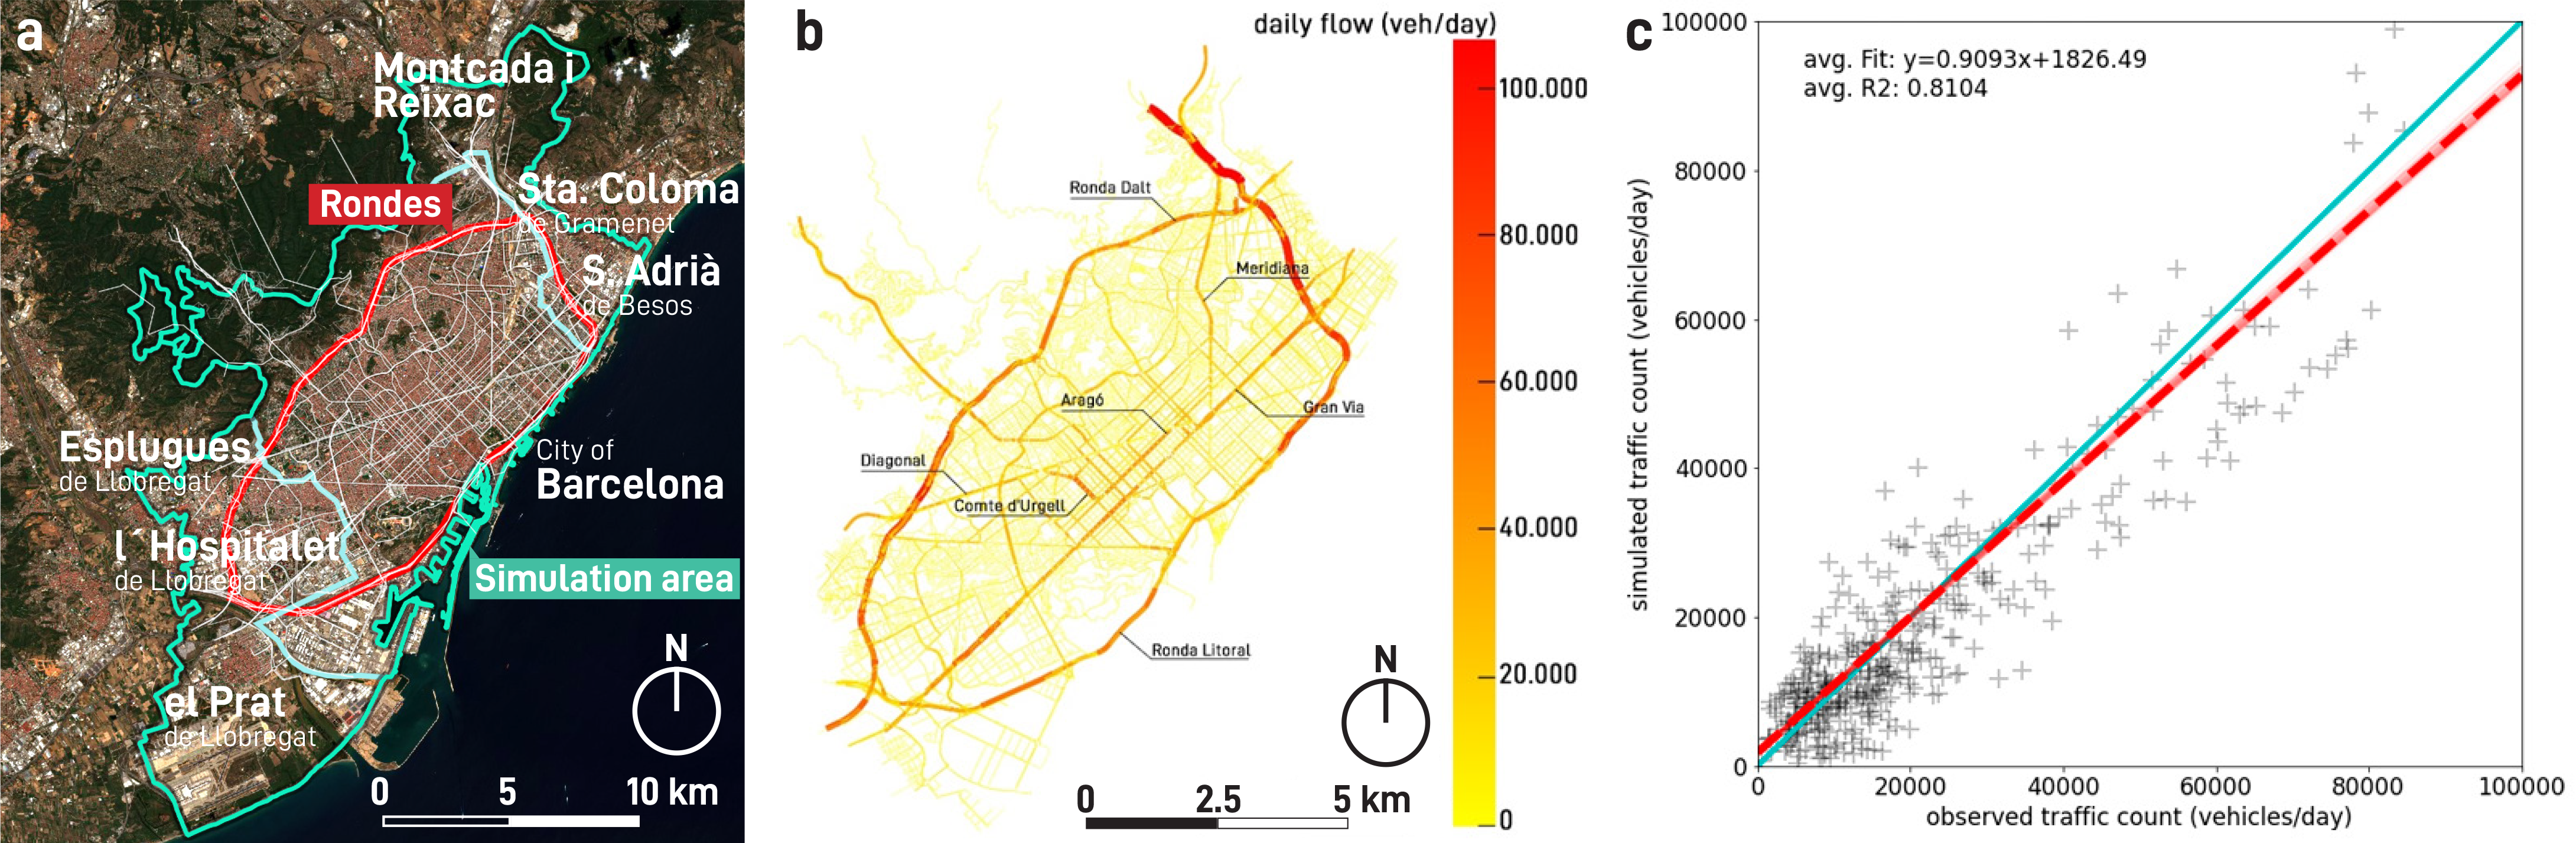
\includegraphics[width=1\textwidth]{LCBM_fig02.jpg}
    % \captionsetup{format=plain, justification=centering} % Center the caption
    \caption{Illustration of the road network used in the base model (adapted from \citep{ArgotaSanchez-Vaquerizo2021}: (\textbf{a}) location and extension, (\textbf{b}) traffic counts results, (\textbf{c}) regression plot comparing real and simulated traffic counts.}
   \label{fig:LCBM_fig02}
\end{figure}

The base model covers the inner part of the Metropolitan Area of Barcelona, roughly defined by the main orbital road of the city (Rondes). However, for a more accurate demand estimation and to avoid simplifications \citep{Tilg2020,Schweizer2021}, the mobility of the much larger entire Metropolitan Region of Barcelona (RMB) has been modelled initially to later crop the area of study corresponding to the metropolitan core (see Table 2 in Argota Sánchez-Vaquerizo, 2021). The model used is based on 24 hours of traffic demand based on real cell phone tracking data totalling 2,063,177 trips in private vehicles in a network made of 2506.03 km of roadways spanning across 182.55 km2, populated by 1,636,762 inhabitants.

Due to the large number of parameters involved and the long run-times, model calibration is challenging \citep{alma990009089600205503}.  The most realistic results are obtained with [74] \citep{ArgotaSanchez-Vaquerizo2021}:
\begin{itemize}
    \item the time step to realistically reproduce the continuous movement of traffic \citep{Lieberman1996} set to 0.25 seconds,
    \item Krauss’ car-following model \citep{Krauss1997} and Erdmann’s lane-changing model \citep{Erdmann2015}, using SUMO’s default parameters,
    \item a rerouting behaviour that is configured such that all vehicles recompute their paths during the simulation (i.e. $device.rerouting.probability = 1$) and with factors in the hierarchy of roads based on the priority values of edges (i.e. $weight.priority-factor = 100$).
\end{itemize}

The initial demand routing is computed using a Direct User Assignment (DUA) \citep{GermanAerospaceCenterDLRandothers2021a}, which is simplistic for large complex traffic scenarios and disregards the changing conditions of traffic throughout the day. SUMO’s duaIterate routine \citep{GermanAerospaceCenterDLRandothers2021e}, then uses an iterative optimization process to dynamically redistribute the traffic realistically and efficiently in a time-dependent way. At every iteration, it computes the lower-cost paths, which are the basis for the following DUA iterations. Particularly, the implemented heuristic dynamic assignment method (iSAR, standing for in-Simulation Adaptive Rerouting) does not seek an immediate Dynamic User Equilibrium (DUE) \citep{GermanAerospaceCenterDLRandothers2021e}. It rather adapts traffic efficiently using a very fast adaptive strategy based on allowing the agents to reroute automatically during the simulation if they find a faster route [74] \citep{ArgotaSanchez-Vaquerizo2021}. As a result, this process approximates the DUE  (i.e. Wardrop’s User Equilibrium) by assuming that traffic will distribute spatially in such a way that no single agent can improve its individual travel time by rerouting \citep{Wardrop1952}. This process also considers a probabilistic component in the routing process to reflect the limited knowledge of agents about the network \citep{Daganzo1977}, and it achieves a Stochastic User Equilibrium \citep{Barcelo2006}. Computing for a driver $d$, the probability $p_d$ to choose a new route with lower cost is based on the travel time of the chosen routes in the previous iteration, and it takes into account the sum of travel times for a set $\mathcal{P}_d$ of known alternative routes and previous probabilities following the method developed by Gawron \citep{Gawron1999}. After each iteration, travel times $\tau_d (x)$  for driver d to complete route x are updated for a given route $x$ following \autoref{eq:LCBM_gawron}:

\begin{align}
   \tau'_d(x) = \begin{cases} \tau_s(x) & \text{if route } x \text{ was simulated} \\ \beta \tau_r(x) + (1 - \beta)\tau_d(x) & \text{otherwise} \end{cases} \label{eq:LCBM_gawron}
\end{align}

Herein, $\tau_s (x)$ is the simulated travel time, $\tau_r (x)$ is the estimated travel time from the simulation for other routes not used in the iteration, and $\beta$ is a remembering factor for scaling the impact of costs of past unused routes. Then, the relative cost difference $\delta_{rs}$ between routes $r$ and $s$ can be computed based on \autoref{eq:LCBM_gawron_delta_rs}:

\begin{align}
   \delta_{rs} = \frac{\tau_d(s) - \tau_d(r)}{\tau_d(s) + \tau_d(r)} \in [-1, 1] & \text{ with }(r,s) \in \mathcal{P}_d \label{eq:LCBM_gawron_delta_rs}
\end{align}

Then, the probabilities for each route can be updated according to \cref{eq:LCBM_gawron_prob_update1,eq:LCBM_gawron_prob_update2}:

\begin{align}
   p'_d(r) = \frac{p_d(r) \left(p_d(r) + p_d(s)\right) \exp\left(\frac{\alpha \delta_{rs}}{1 - \delta_{rs}^2}\right)}{p_d(r) \exp\left(\frac{\alpha \delta_{rs}}{1 - \delta_{rs}^2}\right) + p_d(s)} \label{eq:LCBM_gawron_prob_update1}
\end{align}

\begin{align}
   p'_d(s) = p_d(r) + p_d(s) - p'_d(s) \label{eq:LCBM_gawron_prob_update2}
\end{align}

Herein, $p_d (x)$ and $p'_d (x)$ are the prior and new probabilities to use route $x$, $r$ is the route used in the previous simulation iteration, and $s$ is another route in the set of alternatives $\mathcal{P}_d$. The simulations use SUMO’s default values for Gawron’s parameters, namely $\alpha=0.5$ and $\beta=0.9$.

\subsection{Extension of the base model: fleet composition and emissions}
\label{subsec:LCBM_2.2_ext_base_model}

The initial base model focuses on realistically reproducing the “status quo” and quantifying the traffic behaviour and distribution. It serves as a reference for the what-if analysis making comparisons with alternative scenarios. To improve the capabilities of this simulation in terms of realism, complexity, and environmental effects, this paper expands the base model by considering diverse agents based on the actual fleet composition of the city and an emissions model. Both additions allow taking into account the heterogeneity of agents, and assessing the environmental impact of the interventions, also counterintuitive effects. 

The agents of the urban simulation match the composition of the actual vehicle fleet of the city of Barcelona \citep{Rodriguez-Rey2022,AjuntamentdeBarcelona2017} and the respective emission standards (see \cref{fig:LCBM_fig03}). This provides results in a more accurate picture of traffic in the city by considering different vehicle sizes, speeds, acceleration profiles, and pollution characteristics. To extract the pollutants generated by each type of vehicle and analyse the environmental impact of the different scenarios, the traffic microsimulation is coupled with the software and data module PHEMlight \citep{Hausberger2014}, an instantaneous emission model based on PHEM (Passenger Car and Heavy Duty Emission Model) \citep{Rexeis2014,Hausberger2009}.

\begin{figure}[htbp!]
    \centering
    \includegraphics[width=1\textwidth]{LCBM_fig03.jpg}
    % \captionsetup{format=plain, justification=centering} % Center the caption
    \caption{Estimated fleet composition of the city of Barcelona \citep{Rodriguez-Rey2022,AjuntamentdeBarcelona2017}. General hue represents each type of vehicle, with an increasing level of colour saturation for more polluting classes according to European standards. Normative limit values for carbon monoxide (CO), carbon hydride (HC), nitrogen oxide (NO\textsubscript{X}), and particulate matter (PM\textsubscript{X}) are provided in g/km. The area represents the respective share of these classes. Symbols: (\texttildelow) Euro 0 motorbikes (0.26\%), (§) Euro 1 petrol passenger cars (0.4\%), (*) Euro 2 heavy-duty vehicles (0.2\%).}
   \label{fig:LCBM_fig03}
\end{figure}

PHEMlight calculates at each simulation time step the emissions for each vehicle in two steps. First, the power required by vehicles is computed according to \autoref{eq:LCBM_power}:

\begin{align}
   P_e = \frac{P_{\text{Roll}} + P_{\text{Air}} + P_{\text{Accel}} + P_{\text{Grad}}}{\eta_{\text{gearbox}}} \label{eq:LCBM_power}
\end{align}

Herein, the components of power demand are computed according to \cref{eq:LCBM_P_Roll,eq:LCBM_P_Air,eq:LCBM_P_Accel,eq:LCBM_P_Grad}:

\begin{align}
   P_{\text{Roll}} = g (m_{\text{vehicle}} + m_{\text{load}}) (F_{r0} + F_{r1} \nu + F_{r2} v^4) v \label{eq:LCBM_P_Roll}
\end{align}

\begin{align}
   P_{\text{Air}} = \left(c_d A \frac{\rho}{2} \right) v^3 \label{eq:LCBM_P_Air}
\end{align}

\begin{align}
   P_{\text{Accel}} = (m_{\text{vehicle}} + m_{\text{rot}} + m_{\text{load}}) a v \label{eq:LCBM_P_Accel}
\end{align}

\begin{align}
   P_{\text{Grad}} = 0.01 v (m_{\text{vehicle}} + m_{\text{load}}) G_{\text{road}} \label{eq:LCBM_P_Grad}
\end{align}

with

% Power demands
\begin{itemize}
    \item $P_{\text{Roll}}$: power demand to overcome rolling resistance (W)
    \item $P_{\text{Air}}$: power demand to overcome air resistance (W)
    \item $P_{\text{Grad}}$: power demand to overcome road gradient (W)
    \item $P_{\text{Accel}}$: power demand for acceleration (W)

% Efficiency
    \item $\eta_{\text{gearbox}}$: driver train loss (set to 0.95 as average efficiency)

% Masses
    \item $m_{\text{vehicle}}$, $m_{\text{load}}$: masses of the empty vehicle and its driver, passengers, and/or payload (kg)

% Constants
    \item $g$: gravitational constant (9.81 m/s²)

% Rolling resistance coefficients
    \item $F_{r0}$, $F_{r1}$, $F_{r2}$: rolling resistance coefficients (-, s/m, s$^4$/m$^4$)

% Velocity
    \item $v$: velocity of the vehicle (m/s)

% Air resistance coefficient
    \item $c_d$: air resistance coefficient of the vehicle (-)

% Cross-sectional area
    \item $A$: cross-sectional area (m$^2$)

% Air density
    \item $\rho$: air density (approximately 1.225 kg/m$^3$)

% Acceleration
    \item $a$: acceleration of the vehicle (m/s$^2$)

% Rotational mass
    \item $m_{\text{rot}}$: equivalent rotational mass of accelerated parts (kg)

% Road slope
    \item $G_{\text{road}}$: road slope (\%)
\end{itemize}

Second, PHEMlight computes the emission values from the required power based on the CEPs (Characteristic Emission curves over Power). These curves define emissions as a function of power and are computed using PHEM with representative dynamic real-world driving cycles \citep{Bieker2015}. The emission model distinguishes between different vehicle classes. Using the fleet composition data from the city facilitates more accurate simulations of emissions.

\subsection{Scenarios}
\label{subsec:LCBM_2.3_scenarios}

The initial base model uses a road network created with OpenStreetMap (OSM) data \citep{OpenStreetMap}, obtained through a script based on OSMnx \citep{Boeing2017}. The raw OSM data is transformed into the SUMO network format and manually checked and corrected based on satellite data where necessary and appropriate, to ensure the infrastructure situation of the city is reflected as realistically as possible. Next, a what-if analysis is performed by comparing the effects of different strategies to reduce the street space allocated to motor vehicles. The proposed scenarios are as follows (see \cref{fig:LCBM_fig04}):  

\begin{enumerate}[label=\alph*]
    \item \textbf{Baseline}\textbf{:} This represents the city's infrastructure situation as of early 2021 [74] \citep{ArgotaSanchez-Vaquerizo2021} i.e. before the undergoing massive street redesign and repurposing throughout the city \citep{AjuntamentdeBarcelona2020implementingSuperblocks}.
    \item \textbf{Superblocks} (\emph{Superillas} in Catalan, noted as \emph{superB})\textbf{:} This follows the initial plans envisioned by the City Council of Barcelona and the Agencia d’Ecologia Urbana de Barcelona, aiming to create restricted access inside groups of 3x3 of the existing blocks of the city to enhance active mobility and promote pedestrian activities across the city \citep{Rueda2018}.
    \item \textbf{Green axes} (\emph{Aixos verds} in Catalan, noted as \emph{eixV})\textbf{:} This is the plan currently being implemented by the City Council. It is a variant of the original Superblocks plan. Instead of creating traffic-restricted areas within groups of blocks, this approach aims to transform long streets of the city into continuous traffic-calmed pedestrian-friendly streets across the urban fabric, to create new green areas and enhance citizen activities \citep{AjuntamentdeBarcelona2021c}.
    \item \textbf{No diagonals} (noted as \emph{noDiag})\textbf{:} This is an alternative strategy proposing to close streets based on removing links, which do not follow the regular grid of the city \citep{Cerda1867}. The rationale supporting the closing of diagonal streets and avenues follows several intuitive considerations: (i) the city itself has been calming diagonal streets in the last years \citep{EuropaPress2009}. (ii) It is a feasible and straightforward strategy from the planning and design point of view. (iii) It helps to simplify street intersections. And (iv), it seems to undo shortcuts in the network  (such as diagonal streets), which cause a performance drop due to counterintuitive effects \citep{Braess1969,Sheffi1978}.
    \item \textbf{Hybrid} (noted as \emph{nDeV})\textbf{:} This combines both previous strategies (i.e. green axes and no diagonals). In this scenario, it is possible to verify whether the effects caused by both types of interventions are linear and additive. 
\end{enumerate}

\begin{figure}[htbp!]
    \centering
    \includegraphics[width=1\textwidth]{LCBM_fig04.jpg}
    % \captionsetup{format=plain, justification=centering} % Center the caption
    \caption{Tested strategies for scenarios of vehicular traffic space reduction: (\textbf{a}) baseline, (\textbf{b}) Superblocks, (\textbf{c}) green axes, (\textbf{d}) no diagonals, and (\textbf{e}) hybrid. Streets shown in black are open to all vehicles. Streets shown in green are calmed down or pedestrianized streets and pruned (removed) from the simulation network of motorized traffic.}
   \label{fig:LCBM_fig04}
\end{figure}

For each strategy, a few alternatives are proposed, which differ in the number and capacity of streets closed (see \cref{fig:LCBM_fig05}). For instance, scenarios \emph{noDiag\_103}, \emph{noDiag\_110}, and \emph{noDiag\_122} share the same approach based on removing diagonal streets. However, \emph{noDiag\_122} removes only 0.15\% of the diagonal streets with a higher proportion of single-lane streets, while \emph{noDiag\_103} and \emph{noDiag\_110} go further by closing down 1.29\% and 2.34\%, respectively with a higher proportion of multi-lane streets. The other strategies and respective scenarios follow the same logic (see \cref{tab:LCBM_scenarios_characteristics}).

\begin{table}
\centering
\caption{Main metrics describing the road networks of alternative scenarios considered in the study. Differences between the length of streets and the length of lanes reflect the existence of streets with more than one lane.}
\label{tab:LCBM_scenarios_characteristics}
\resizebox{\linewidth}{!}{%
\begin{tblr}{
  colsep = 2pt,
  row{even} = {c},
  cell{1}{1} = {r=2}{},
  row{3} = {c},
  row{5} = {c},
  row{7} = {c},
  row{9} = {c},
  row{11} = {c},
  cell{1}{1} = {r=2}{},
  cell{1}{2} = {r=2}{c},
  cell{1}{3} = {r=2}{c},
  cell{1}{4} = {r=2}{},
  cell{1}{5} = {r=2}{c},
  cell{1}{6} = {r=2}{c},
  cell{1}{7} = {r=2}{c},
  cell{1}{8} = {c=5}{c},
  hline{1,13} = {-}{0.08em},
  hline{2} = {8-12}{},
  hline{3} = {-}{},
  % width = \linewidth,
  % Specify fixed width for columns 2 to 12
  colspec = {Q[wd=2cm] *{10}{Q[wd=1.05cm]} Q[wd=0.95cm]}
}
\textbf{Alternative}   & \rotcell{\textbf{Asphalt surface}\\\textbf{(km\textsuperscript{2})}} & \rotcell{\textbf{Number of edges}} & \rotcell{\textbf{Number of nodes}} & \rotcell{\textbf{Total length of streets (km)}} & \rotcell{\textbf{Total length of lanes (km)}} & \rotcell{\textbf{Average number of lanes closed in street sections}} & \textbf{\% Difference compared to \textit{baseline\_000} (=100\%)} &                                                                    &                                                                    &                                                                                      &                                                                                   \\
                       &                                                                          &                                                        &                                                        &                                                                                 &                                                                              &                                                                                                                & \rotcell{\textbf{Asphalt surface}} & \rotcell{\textbf{Number of edges}} & \rotcell{\textbf{Number of nodes}} & \rotcell{\textbf{Total length of streets}} & \rotcell{\textbf{Total length of lanes}} \\
\textbf{baseline\_000} & 12.86                                                                    & 25307                                                  & 13993                                                  & 2506                                                                            & 3673                                                                         & ~                                                                                                              &                                                                    &                                                                    &                                                                    &                                                                             &                                                                          \\
\textbf{noDiag\_103}   & 12.69                                                                    & 25106                                                  & 13954                                                  & 2486                                                                            & 3626                                                                         & 2.40                                                                                                           & -1.29                                                              & -0.79                                                              & -0.28                                                              & -0.79                                                                       & -1.29                                                                    \\
\textbf{noDiag\_110}   & 12.56                                                                    & 24930                                                  & 13913                                                  & 2469                                                                            & 3587                                                                         & 2.31                                                                                                           & -2.34                                                              & -1.49                                                              & -0.57                                                              & -1.48                                                                       & -2.34                                                                    \\
\textbf{noDiag\_122}   & 12.83                                                                    & 25281                                                  & 13988                                                  & 2502                                                                            & 3666                                                                         & 1.93                                                                                                           & -0.20                                                              & -0.10                                                              & -0.04                                                              & -0.15                                                                       & -0.19                                                                    \\
\textbf{eixV\_002}     & 12.80                                                                    & 25218                                                  & 13966                                                  & 2497                                                                            & 3658                                                                         & 1.59                                                                                                           & -0.41                                                              & -0.35                                                              & -0.19                                                              & -0.38                                                                       & -0.41                                                                    \\
\textbf{eixV\_011}     & 12.56                                                                    & 24762                                                  & 13881                                                  & 2453                                                                            & 3589                                                                         & 1.60                                                                                                           & -2.30                                                              & -2.15                                                              & -0.80                                                              & -2.11                                                                       & -2.30                                                                    \\
\textbf{superB\_009}   & 12.16                                                                    & 23990                                                  & 13527                                                  & 2378                                                                            & 3474                                                                         & 1.56                                                                                                           & -5.42                                                              & -5.20                                                              & -3.33                                                              & -5.10                                                                       & -5.42                                                                    \\
\textbf{superB\_010}   & 12.04                                                                    & 23815                                                  & 13430                                                  & 2360                                                                            & 3440                                                                         & 1.60                                                                                                           & -6.36                                                              & -5.90                                                              & -4.02                                                              & -5.82                                                                       & -6.36                                                                    \\
\textbf{nDeV\_102}     & 12.51                                                                    & 24852                                                  & 13884                                                  & 2461                                                                            & 3574                                                                         & 2.19                                                                                                           & -2.69                                                              & -1.80                                                              & -0.78                                                              & -1.80                                                                       & -2.69                                                                    \\
\textbf{nDeV\_111}     & 12.27                                                                    & 24415                                                  & 13781                                                  & 2418                                                                            & 3505                                                                         & 1.91                                                                                                           & -4.59                                                              & -3.52                                                              & -1.52                                                              & -3.52                                                                       & -4.59                                                                    
\end{tblr}
}
\end{table}


\begin{figure}[htbp!]
    \centering
    \includegraphics[width=1\textwidth]{LCBM_fig05.jpg}
    % \captionsetup{format=plain, justification=centering} % Center the caption
    \caption{City maps of the selected alternative scenarios: (\textbf{a}) \emph{baseline}, (\textbf{b}) \emph{eixV\_002}, (\textbf{c}) \emph{superB\_009}, and (\textbf{d}) \emph{superB\_010}. In green, the closed roadways to traffic are highlighted; in black, open roadways to general traffic are shown. The rectangles below each subfigure display a zoom of the central part of the city most affected by the various road closures considered. (For all alternatives, see \cref{fig:LCBM_fig_map_01}).}
   \label{fig:LCBM_fig05}
\end{figure}

Each alternative scenario uses the same initial traffic demand determined for the baseline scenario (\emph{baseline\_000}) after having been adapted to the new pruned network (see \cref{fig:LCBM_fig06}) \citep{GermanAerospaceCenterDLRandothers2021}. In very few cases, if a route falls almost entirely within a part of the street network that has been closed down in such a way that there are no feasible alternatives for rebuilding the route in the new network, this route may disappear from the demand, resulting in a slightly lower total number of trips for the scenario (around 1\%) (see \cref{fig:LCBM_fig07}a). Generally, however, the trips are adapted to the new network by rerouting and by adjusting origin and destinations slightly, if they fall within a closed street.

\begin{figure}[htbp!]
    \centering
    \includegraphics[width=1\textwidth]{LCBM_fig06.jpg}
    % \captionsetup{format=plain, justification=centering} % Center the caption
    \caption{Data flow used for the model building and evaluation of results. Real-world cell phone tracks are used to estimate travel demand for the simulations. Later, simulation results are validated with measured real-world traffic.}
   \label{fig:LCBM_fig06}
\end{figure}

\section{Results}
\label{sec:LCBM_3_results}

The goal of simulating different scenarios is to prove that there are interventions that can improve the general performance of traffic in the city. Each scenario is tested in 25 iterations to approximate the DUE following the stochastic dynamic assignment method “in-Simulation Adaptive Routing” (iSAR) [74], [85] \citep{ArgotaSanchez-Vaquerizo2021,GermanAerospaceCenterDLRandothers2021e}. For the analysis of the results, the first iteration is considered to be a “warming up”, and hence, it is discarded.

The microscopic model simulates the movement of the vehicles across the network during an entire working day, recording at each step their position, speed, and acceleration \citep{Helbing2010}. It also determines their energy consumption and pollutant emissions based on the coupling with the instantaneous emission model \citep{Hausberger2014}. Hence, the simulations provide three types of metrics (see \cref{tab:appendix_LCBM_eval_metrics}):
\begin{itemize}
    \item \textbf{Simulation performance:} This is related directly to the simulation parameters and initialization. The \emph{vehicles loaded factor} and \emph{number of vehicles inserted} express the variability of the number of vehicles effectively inserted in the simulation, assuming the same transportation demand in all scenarios. The small differences result from pruning the network, slight variations of demand, and the accordingly changing levels of saturation. The \emph{percentage of teleports} is related to the level of saturation of the network \citep{GermanAerospaceCenterDLRandothers2021teleporting}. A smaller number of teleports is a sign of better simulation performance.
    \item \textbf{Efficiency:} These metrics focus on a cost-related perspective within an economic perception of resources. They follow the common economic logic of minimizing times (e.g. \emph{departure delay}, \emph{trip duration}, \emph{time loss}, \emph{waiting time}) and/or distances (\emph{trip length}), or maximizing speeds \citep{GermanAerospaceCenterDLRandothers}.
    \item \textbf{Environmental:} These metrics are obtained from the instantaneous emission model PHEMlight \citep{Hausberger2014}, which is applied to all vehicles in the simulation. In general, these are aimed to be as small as possible, no matter whether they refer to fuel consumption (\emph{total fuel}) or the emission of pollutants (carbon dioxide —\emph{CO\textsubscript{2}}—, carbon monoxide —\emph{CO}—, carbon hydride —\emph{HC}—, nitrogen oxide —\emph{NO\textsubscript{X}}—, and particulate matter —\emph{PM\textsubscript{X}}—).  
\end{itemize}

% \begin{figure}[htbp!]
%     \centering
%     \begin{threeparttable}
%         \includegraphics[width=1\textwidth]{LCBM_fig07.jpg}
%         % \captionsetup{format=plain, justification=centering} % Center the caption
%         \caption{Histograms of results from microsimulations of all scenarios. Similar colours represent scenarios with the same strategy. A dotted hatch indicates evidence for the non-normality of the distribution of simulation data. Overall, scenario \emph{eixV\_002} shows better performance in all the metrics. A stripped hatch indicates evidence for the bimodality of the distribution. On top of each subplot, statistically significant ($alpha=0.05$) differences with regard to the baseline scenario are highlighted as result of the post hoc test with p-values adjusted for the many comparisons following [102]\citep{Benjamini1995} (*: $0.05 => p-value > 0.01$; **: $0.01=> p-value > 0.001$; ***: $0.001=> p-value > 0.0001$; ****: $p-value<=0.0001$). (For complete metrics see Table B3 and Table B4).}
%         \label{fig:LCBM_fig07}
%     \end{threeparttable}
% \end{figure}

\begin{figure}[htbp!]
    \centering
    \includegraphics[width=1\textwidth]{LCBM_fig07.jpg}
    % \captionsetup{format=plain, justification=centering} % Center the caption
    \caption*{(Description in the following page.)}
\end{figure}
\captionof{figure}[Caption of \cref{fig:LCBM_fig07} in the previous page]{(\cref{fig:LCBM_fig07} in the previous page) Histograms of results from microsimulations of all scenarios. Similar colours represent scenarios with the same strategy. A dotted hatch indicates evidence for the non-normality of the distribution of simulation data. Overall, scenario \emph{eixV\_002} shows better performance in all the metrics. A stripped hatch indicates evidence for the bimodality of the distribution. On top of each subplot, statistically significant ($alpha=0.05$) differences with regard to the baseline scenario are highlighted as result of the post hoc test with p-values adjusted for the many comparisons following \citep{Benjamini1995} (*: $0.05 => p-value > 0.01$; **: $0.01=> p-value > 0.001$; ***: $0.001=> p-value > 0.0001$; ****: $p-value<=0.0001$). (For complete metrics see \cref{tab:appendix_LCBM_all_metrics_all_scenarios,tab:appendix_LCBM_all_results_post_hocs}).}
\label{fig:LCBM_fig07}


% Reset paragraph indentation after captionof
\setlength{\parindent}{1em}

The diversity of metrics allows one to assess the outcomes of the different scenarios based on various goals and optimization criteria, which are not necessarily mutually aligned. Additionally, they allow for non-linear trade-offs between purely efficiency-oriented optimization criteria, energy consumption and pollutants emissions.

The aggregated analysis of the metrics resulting from the simulations shows a characteristic grouping, with stronger correlation levels among the metrics belonging to the same type (see \cref{fig:LCBM_fig08}).

\begin{figure}[htbp!]
    \centering
    \includegraphics[width=0.65\textwidth]{LCBM_fig08.jpg}
    % \captionsetup{format=plain, justification=centering} % Center the caption
    \caption{Matrix of correlations between the considered metrics. Metrics belonging to the same domain (i.e. efficiency and environmental) are highly correlated. Still, CO\textsubscript{2} emissions are the environmental metric most highly correlated to efficiency factors.}
   \label{fig:LCBM_fig08}
\end{figure}

The analysis of the results of our simulations focuses on two main points: (i) the stability and characterization of the simulation outcomes for the same scenario across its multiple iterations, and (ii) the comparison of the results between the baseline scenario and the proposed alternatives. Respectively, this is similar to the logic of A/A testing or a sensitivity analysis for assessing the internal variability of a given scenario, and A/B testing, i.e. what-if analysis for measuring the effects of the different interventions in each alternative scenario \citep{Rizzi2009,Kohavi2017,Fu2020,Carlino2022}.  Additionally, the experiment accounts for the differences between aggregated effects at the trips level, and local effects at the streets level (see \cref{subsec:LCBM_4.3_sys_stability}).

\subsection{Inner characterization}
\label{subsec:LCBM_3.1_inner_characterization}

First, each scenario is analysed independently, to gain an understanding of the stability and predictability of results. This serves to deliver insights into the different regimes, their equilibrium states, and their characteristics. To study the stability of the system and also of the applicability of many statistical tests, it is necessary to check for normally distributed data, which is particularly important considering the relatively small sample size ($n=24$).

In most scenarios, the results from the Shapiro-Wilk test for normality [106] \citep{Shapiro1965} do not show statistically significant evidence for non-normality for the analysed variables. Given the relatively small sample size ($n = 24$), the threshold of the p-value to reject the null hypothesis is set at 0.1 \citep{Royall1986}. However, scenarios \emph{baseline\_000}, \emph{eixV\_002}, and \emph{nDeV\_102} show evidence for a significant departure from normality \citep{Wasserstein2016,Gomez-de-Mariscal2021} (see \cref{fig:LCBM_fig07,tab:appendix_LCBM_shapiro}).

The evidence for non-normality of some of the distributions in some scenarios and the presence of two apparent peaks (see \cref{fig:LCBM_fig07}) suggest the existence of some degree of multimodality in the microsimulation results. Hence, to complement the normality test, unimodality is checked, using Hartigan’s Dip Test \citep{Hartigan1985,Muldal2019}. This test compares the distance between the empirical cumulative distribution function (eCDF) $F$ and the well-characterized CDF of a set $\mathbb{U}$ of unimodal distributions according to \cref{eq:LCBM_dip_test}:

\begin{align}
   \text{dip}(F) = d_\infty (F, U) = \min_{U \in \mathbb{U}} \|F - U\|_\infty \label{eq:LCBM_dip_test}
\end{align}

Here, the dip of the eCDF $F$ corresponds approximately to the distance of the infinity norm between $F$ and $\mathbb{U}$ (also called supremum norm).

For scenario \emph{baseline\_000}, the results from the dip test show evidence for bimodality (i.e. $p<0.05$) in most of the metrics (such as \emph{average trip duration}, \emph{average trip length}, \emph{average time loss}, \emph{average waiting time},  and all environmental metrics) (see \cref{fig:LCBM_fig07}). The bimodality of the distributions for \emph{baseline\_000} may be interpreted as the existence of two equilibria for traffic in the city, i.e. the resulting equilibrium may be significantly different on different days as a result of small variations (see \cref{subsec:LCBM_4.3_sys_stability}). Some interventions in the network seem to even attenuate these bimodal tendencies at an aggregated level like in the case of the scenario \emph{eixV\_002} (see \cref{fig:LCBM_fig07,tab:appendix_LCBM_dip_test}).

Despite the multiple iterations and their stochastic variations of variables, most scenarios show stable results within a range of ±3 standard deviations, following the six sigma (6$\sigma$) criteria \citep{Smith1993,Montgomery2008}. This is aligned with the results from the iSAR algorithm observed in the base model [74] \citep{ArgotaSanchez-Vaquerizo2021} and suggests that the differences between scenarios are the main explanation for the differences in the results. 

\subsection{Comparison between scenarios}
\label{subsec:LCBM_3.2_comp_scenarios}

A linear regression is made to estimate each factor level (i.e. metrics) (see \cref{tab:appendix_LCBM_all_metrics_all_scenarios}). Furthermore, post hoc tests are performed (see \cref{tab:appendix_LCBM_all_results_post_hocs}) to assess whether the mean results of the simulations for each scenario significantly differ from the \emph{baseline} \citep{Lee2013,Jafari2019}. Note that regression analysis was chosen to determine levels of significance and get well-interpretable and explainable results. For other purposes such as prediction, other methods such as machine learning may be better suited \citep{Mirzahossein2022,Zargari2022}.

As mentioned, the pruning interventions may slightly reduce the total number of programmed trips (see \cref{fig:LCBM_fig07}a) due to a lack of alternative routes. However, this does not imply that the total number of vehicles effectively inserted is necessarily smaller (see \cref{fig:LCBM_fig07}b). Overall, this number fluctuates within a range of ±2.5\%. The scenarios based on closing down emph{diagonal} streets (\emph{noDiag\_***}) tend to differ little from the \emph{baseline} scenario. The \emph{Superblocks} (\emph{superB\_***}) and the \emph{hybrid} (\emph{nDeV\_***}) scenarios insert slightly fewer vehicles, while the \emph{green axes} scenarios (\emph{eixV\_***}) are able to cope with even more vehicles than the \emph{baseline} (e.g.  \emph{eixV\_002}), probably due to better traffic performance. In general, these different trends of traffic performance and their dependence on the strategies are mirrored by the rest of the metrics.

The number of teleports, which is a metric of the general level of realism and performance of the microsimulations, tends to be similar or smaller than in the \emph{baseline} for all scenarios except for the \emph{Superblocks} cases (\emph{superB\_***}) (see \cref{fig:LCBM_fig07}c). Fewer teleports imply that the overall congestion levels are lower and the simulated traffic flow is smoother.

Regarding the efficiency-oriented metrics, in general, it can be assumed that shorter travel times and distances as well as higher speeds are preferred by most citizens. Closing down \emph{diagonal} streets (\emph{noDiag\_***}), creating \emph{green axes} (\emph{eixV\_***}), and a \emph{hybrid} combination of both strategies (\emph{nDeV\_***}) have, in general, positive effects on the traffic performance by reducing both average trip times (\cref{fig:LCBM_fig07} d, e, h, i) and travelled distances (\cref{fig:LCBM_fig07}f). This allows for higher average speeds (\cref{fig:LCBM_fig07}g). Only the \emph{average departure delay} seems to slightly increase for the \emph{noDiag\_103} scenario. However, scenarios following the \emph{Superblocks} approach (\emph{superB\_***}) have opposite effects by incrementing travel times and distances while reducing the average speed.

Similar general trends can be identified for the environmental metrics. Pruning strategies based on closing down \emph{diagonal} streets, \emph{green axes}, or a \emph{hybrid} combination of both reduce emissions and fuel consumption, while the opposite is the case in the simulated \emph{Superblocks} scenarios (see \cref{fig:LCBM_fig07} j-o).

Despite the differences in the results across scenarios, not all are different from the baseline in terms of statistical significance (see \cref{tab:appendix_LCBM_all_metrics_all_scenarios,tab:appendix_LCBM_all_results_post_hocs}). Only one of the green axes scenarios (\emph{eixV\_002}), and the two scenarios based on the \emph{Superblock} strategy (\emph{superB\_009} and \emph{superB\_010}) show statistically significant differences compared to the \emph{baseline} situation. As previously noted, the \emph{eixV\_002} scenario improves the general performance of traffic, shortening the median \emph{travel duration} by 14.07\% and making the median trip 3.51\% shorter. Median emissions and fuel consumption are reduced as well by about 7\%, as are CO\textsubscript{2} emissions by 7.13\%. Conversely, the two simulated \emph{Superblocks} scenarios, namely \emph{superB\_009} and \emph{superB\_010}, increase the median \emph{average trip duration} between 4.56\% and 16.43\% (about 80-290 s more) and the median \emph{trip length} between 1.29\% and 3.21\% (about 100-250 m longer). Emissions and fuel consumption are only significantly larger for the scenario \emph{superB\_010}, with a rise of about 5\% (see \cref{tab:LCBM_selection_results}).

As a final remark, the improvement in traffic performance in scenario \emph{eixV\_002}  and its unimodality come with a trade-off, namely an increase in the variance of results (+11.86\% for travel times, +2.62\% of route lengths, and about +20\% for all environmental metrics). In contrast, the \emph{Superblocks} interventions, while featuring the worst-performing traffic, they tend to have a smaller variance (see \cref{tab:LCBM_selection_results}).

% \usepackage{color}
% \usepackage{tabularray}
\definecolor{SnowyMint}{rgb}{0.78,1,0.784}
\definecolor{MonaLisa}{rgb}{1,0.592,0.592}
\begin{table}
\centering
\caption{Effect analysis in selected metrics. Scenarios that are significantly better than the baseline are presented in green. Significantly worse scenarios are shown in red. Scenario \emph{eixV\_002}, which consists of a moderate closing to general vehicular traffic of a few streets from the regular urban fabric for the creation of green axes across the city, shows consistently the best results for all types of metrics. (For a complete comparison between scenarios, see \cref{tab:appendix_LCBM_all_results_post_hocs}). }
\label{tab:LCBM_selection_results}
\resizebox{\linewidth}{!}{%
\begin{tblr}{
  colsep = 3pt,
  row{4} = {SnowyMint},
  row{5} = {MonaLisa},
  row{6} = {MonaLisa},
  row{8} = {SnowyMint},
  row{9} = {MonaLisa},
  row{10} = {MonaLisa},
  row{12} = {SnowyMint},
  row{13} = {MonaLisa},
  row{14} = {MonaLisa},
  row{16} = {SnowyMint},
  row{17} = {MonaLisa},
  row{18} = {MonaLisa},
  row{20} = {SnowyMint},
  row{21} = {MonaLisa},
  row{22} = {MonaLisa},
  cell{1}{5} = {c=3}{},
  cell{1}{9} = {c=3}{},
  cell{3}{2} = {r},
  cell{3}{3} = {r},
  cell{3}{4} = {r},
  cell{3}{12} = {r=4}{t},
  cell{4}{2} = {r},
  cell{4}{3} = {r},
  cell{4}{4} = {r},
  cell{4}{5} = {r},
  cell{4}{6} = {r},
  cell{4}{7} = {r},
  cell{4}{9} = {r},
  cell{4}{10} = {r},
  cell{4}{11} = {r},
  cell{5}{2} = {r},
  cell{5}{3} = {r},
  cell{5}{4} = {r},
  cell{5}{5} = {r},
  cell{5}{6} = {r},
  cell{5}{7} = {r},
  cell{5}{9} = {r},
  cell{5}{10} = {r},
  cell{5}{11} = {r},
  cell{6}{2} = {r},
  cell{6}{3} = {r},
  cell{6}{4} = {r},
  cell{6}{5} = {r},
  cell{6}{6} = {r},
  cell{6}{7} = {r},
  cell{6}{9} = {r},
  cell{6}{10} = {r},
  cell{6}{11} = {r},
  cell{7}{2} = {r},
  cell{7}{3} = {r},
  cell{7}{4} = {r},
  cell{7}{12} = {r=4}{t},
  cell{8}{2} = {r},
  cell{8}{3} = {r},
  cell{8}{4} = {r},
  cell{8}{5} = {r},
  cell{8}{6} = {r},
  cell{8}{7} = {r},
  cell{8}{9} = {r},
  cell{8}{10} = {r},
  cell{8}{11} = {r},
  cell{9}{2} = {r},
  cell{9}{3} = {r},
  cell{9}{4} = {r},
  cell{9}{5} = {r},
  cell{9}{6} = {r},
  cell{9}{7} = {r},
  cell{9}{9} = {r},
  cell{9}{10} = {r},
  cell{9}{11} = {r},
  cell{10}{2} = {r},
  cell{10}{3} = {r},
  cell{10}{4} = {r},
  cell{10}{5} = {r},
  cell{10}{6} = {r},
  cell{10}{7} = {r},
  cell{10}{9} = {r},
  cell{10}{10} = {r},
  cell{10}{11} = {r},
  cell{11}{2} = {r},
  cell{11}{3} = {r},
  cell{11}{4} = {r},
  cell{11}{12} = {r=4}{t},
  cell{12}{2} = {r},
  cell{12}{3} = {r},
  cell{12}{4} = {r},
  cell{12}{5} = {r},
  cell{12}{6} = {r},
  cell{12}{7} = {r},
  cell{12}{9} = {r},
  cell{12}{10} = {r},
  cell{12}{11} = {r},
  cell{13}{2} = {r},
  cell{13}{3} = {r},
  cell{13}{4} = {r},
  cell{13}{5} = {r},
  cell{13}{6} = {r},
  cell{13}{7} = {r},
  cell{13}{9} = {r},
  cell{13}{10} = {r},
  cell{13}{11} = {r},
  cell{14}{2} = {r},
  cell{14}{3} = {r},
  cell{14}{4} = {r},
  cell{14}{5} = {r},
  cell{14}{6} = {r},
  cell{14}{7} = {r},
  cell{14}{9} = {r},
  cell{14}{10} = {r},
  cell{14}{11} = {r},
  cell{15}{2} = {r},
  cell{15}{3} = {r},
  cell{15}{4} = {r},
  cell{15}{12} = {r=4}{t},
  cell{16}{2} = {r},
  cell{16}{3} = {r},
  cell{16}{4} = {r},
  cell{16}{5} = {r},
  cell{16}{6} = {r},
  cell{16}{7} = {r},
  cell{16}{9} = {r},
  cell{16}{10} = {r},
  cell{16}{11} = {r},
  cell{17}{2} = {r},
  cell{17}{3} = {r},
  cell{17}{4} = {r},
  cell{17}{5} = {r},
  cell{17}{6} = {r},
  cell{17}{7} = {r},
  cell{17}{9} = {r},
  cell{17}{10} = {r},
  cell{17}{11} = {r},
  cell{18}{2} = {r},
  cell{18}{3} = {r},
  cell{18}{4} = {r},
  cell{18}{5} = {r},
  cell{18}{6} = {r},
  cell{18}{7} = {r},
  cell{18}{9} = {r},
  cell{18}{10} = {r},
  cell{18}{11} = {r},
  cell{19}{2} = {r},
  cell{19}{3} = {r},
  cell{19}{4} = {r},
  cell{19}{12} = {r=4}{t},
  cell{20}{2} = {r},
  cell{20}{3} = {r},
  cell{20}{4} = {r},
  cell{20}{5} = {r},
  cell{20}{6} = {r},
  cell{20}{7} = {r},
  cell{20}{9} = {r},
  cell{20}{10} = {r},
  cell{20}{11} = {r},
  cell{21}{2} = {r},
  cell{21}{3} = {r},
  cell{21}{4} = {r},
  cell{21}{5} = {r},
  cell{21}{6} = {r},
  cell{21}{7} = {r},
  cell{21}{9} = {r},
  cell{21}{10} = {r},
  cell{21}{11} = {r},
  cell{22}{2} = {r},
  cell{22}{3} = {r},
  cell{22}{4} = {r},
  cell{22}{5} = {r},
  cell{22}{6} = {r},
  cell{22}{7} = {r},
  cell{22}{9} = {r},
  cell{22}{10} = {r},
  cell{22}{11} = {r},
  hline{1,23} = {-}{0.08em},
  hline{2} = {5-7,9-11}{},
  hline{3} = {-}{},
}
\textbf{Scenario}      & \textbf{Mean} & \textbf{Median} & \textbf{Std.} & {\% Difference \\from \textit{baseline\_000 }} &                 &               &  & {Absolute difference \\from \textit{baseline\_000}} &                 &               & \textbf{Metric}                                                      \\
                       &               &                 &               & \textbf{Mean}                                  & \textbf{Median} & \textbf{Std.} &  & \textbf{Mean}                                       & \textbf{Median} & \textbf{Std.} &                                                                      \\
\textbf{baseline\_000} & 1745.36       & 1773.55         & 193.07        &                                                &                 &               &  &                                                     &                 &               & {\textbf{Avg. }\\\textbf{trip duration }\\\textbf{(s)}}              \\
\textbf{eixV\_002}     & 1593.83       & 1523.98         & 215.96        & -8.68                                          & -14.07          & 11.86         &  & -151.53                                             & -249.57         & 22.89         &                                                                      \\
\textbf{superB\_009}   & 1889.19       & 1854.34         & 208.31        & 8.24                                           & 4.56            & 7.89          &  & 143.84                                              & 80.8            & 15.24         &                                                                      \\
\textbf{superB\_010}   & 2023.96       & 2064.92         & 153.07        & 15.96                                          & 16.43           & -20.72        &  & 278.6                                               & 291.38          & -40           &                                                                      \\
\textbf{baseline\_000} & 7788.56       & 7818.74         & 201.35        &                                                &                 &               &  &                                                     &                 &               & {\textbf{Avg. }\\\textbf{trip length }\\\textbf{(m)}}                \\
\textbf{eixV\_002}     & 7613.98       & 7544.27         & 206.62        & -2.24                                          & -3.51           & 2.62          &  & -174.58                                             & -274.48         & 5.27          &                                                                      \\
\textbf{superB\_009}   & 7937.22       & 7919.5          & 191.75        & 1.91                                           & 1.29            & -4.77         &  & 148.66                                              & 100.76          & -9.6          &                                                                      \\
\textbf{superB\_010}   & 8061.96       & 8072.36         & 127.97        & 3.51                                           & 3.24            & -36.44        &  & 273.4                                               & 253.62          & -73.38        &                                                                      \\
\textbf{baseline\_000} & 5770.64       & 5819.84         & 303.21        &                                                &                 &               &  &                                                     &                 &               & {\textbf{Total CO2 }\\\textbf{(tons/day)}}                           \\
\textbf{eixV\_002}     & 5527.05       & 5405.13         & 366.37        & -4.22                                          & -7.13           & 20.83         &  & -243.59                                             & -414.71         & 63.16         &                                                                      \\
\textbf{superB\_009}   & 5923.91       & 5849.06         & 367.12        & 2.66                                           & 0.5             & 21.08         &  & 153.28                                              & 29.22           & 63.91         &                                                                      \\
\textbf{superB\_010}   & 6117.93       & 6137.63         & 273.43        & 6.02                                           & 5.46            & -9.82         &  & 347.3                                               & 317.79          & -29.78        &                                                                      \\
\textbf{baseline\_000} & 25.53         & 25.75           & 1.37          &                                                &                 &               &  &                                                     &                 &               & {\textbf{Total NOx }\\\textbf{(tons/day)}}                           \\
\textbf{eixV\_002}     & 24.43         & 23.87           & 1.65          & -4.31                                          & -7.29           & 20.42         &  & -1.1                                                & -1.88           & 0.28          &                                                                      \\
\textbf{superB\_009}   & 26.2          & 25.87           & 1.66          & 2.62                                           & 0.46            & 21.22         &  & 0.67                                                & 0.12            & 0.29          &                                                                      \\
\textbf{superB\_010}   & 27.17         & 27.24           & 1.24          & 6.43                                           & 5.8             & -9.28         &  & 1.64                                                & 1.49            & -0.13         &                                                                      \\
\textbf{baseline\_000} & 2.28          & 2.3             & 0.12          &                                                &                 &               &  &                                                     &                 &               & {\textbf{Total fuel }\\\textbf{(millions }\\\textbf{of litres/day)}} \\
\textbf{eixV\_002}     & 2.19          & 2.14            & 0.15          & -4.25                                          & -7.18           & 20.87         &  & -0.1                                                & -0.17           & 0.03          &                                                                      \\
\textbf{superB\_009}   & 2.35          & 2.32            & 0.15          & 2.7                                            & 0.52            & 21.16         &  & 0.06                                                & 0.01            & 0.03          &                                                                      \\
\textbf{superB\_010}   & 2.42          & 2.43            & 0.11          & 6.07                                           & 5.51            & -9.77         &  & 0.14                                                & 0.13            & -0.01         &                                                                      
\end{tblr}
}
\end{table}

\section{Discussion}
\label{sec:LCBM_4_discussion}

Below several problems deserve to be discussed further. These include particular, also counterintuitive, effects related to complex systems, some of which are connected to the Price of Anarchy (\cref{subsec:LCBM_4.1_counter_effects}), or system stability (\cref{subsec:LCBM_4.3_sys_stability}), which may support smart planning (\cref{subsec:LCBM_4.2_close_smart}). Finally, some higher-level considerations regarding political issues in city planning and their overall impacts on society are reflected upon (\cref{subsec:LCBM_4.4_policy,subsec:LCBM_4.5_societal_impact}).

\subsection{Using counterintuitive effects}
\label{subsec:LCBM_4.1_counter_effects}

Braess’ Paradox was formulated a long time ago \citep{Braess1969}. Similarly, Daganzo’s Paradox was proposed as an equivalent for dynamic counterintuitive effect for stochastic models \citep{Sheffi1978}. Accordingly, it is theoretically possible that adding infrastructure can reduce traffic performance. While the practical relevance of this theoretically postulated circumstance was initially not clear, the phenomenon has actually been observed in real life in some places \citep{Baker2009,Chung2012,Knodel1969,Kolata1990,Youn.etal.2008,Cairns.etal1998,Cairns2002}. The possibility to use this counterintuitive effect to produce beneficial planning and policy-making outcomes, however, is still underexplored. While these paradoxes are not formally demonstrated in this article, the simulation results seem to be aligned with these counterintuitive effects. However, exploiting these phenomena face two main challenges: (i) a technical one, and (ii) a cognitive and a communication one. To address these challenges, suitable simulation and visualization tools are needed.

\subsection{Closing down roads smartly}
\label{subsec:LCBM_4.2_close_smart}

The detection of these paradoxes in a big street network is a complex mathematical and computational problem \citep{Bagloee2019}, which is related to the challenge of the traffic assignment problem \citep{Beckmann1956} and the “Price of Anarchy” \citep{Roughgarden2005}. These are paradigms that articulate performance losses caused by selfish routing decisions, i.e. individually optimal but noncooperative \citep{Roughgarden2005}, or queue spillback \citep{Daganzo1998}. For realistic road networks, analytical formulas for these effects are largely lacking, such that computationally costly simulations are the only alternative, which are laborious to set up, calibrate, and evaluate. Hence, it is complicated to simulate these scenarios and even harder to capture the conditions that lead to these effects and spot them, as everything depends on the complex interactions of many agents. Furthermore, from the cognitive and communication perspective, due to their counterintuitive nature, once these effects have been identified, it may still be challenging to turn the findings into accepted policies and to organize the necessary support for them. 

This two-fold difficulty makes urban digital twins a valuable development. On the one hand, they overcome previous limitations of urban simulations with new modelling approaches that can capture, test, and interactively demonstrate alternative scenarios of urban dynamics more realistically and more accurately. On the other hand, these frameworks may help to raise awareness of the complexity of urban systems, while facilitating policy information and decision-making by helping to envision complex scenarios \citep{Borning2008,Bettencourt2019}.

The analysis of our results suggests that the type and location of a street seem to matter more than just the raw amount of meters of removed road sections or the number of lanes when it comes to strategically improving mobility by closing streets. Additionally and connected to this, closing more streets after a tipping point has been reached is detrimental (e.g., \emph{eixV\_002} vs \emph{eixV\_011}). Therefore, a one-fits-all approach falls short. Removing complex and redundant intersections, such as those with more than four convergent streets, seems to help up to a certain point. However, an extensive and uniform closure of streets such as the proposed by the Superblocks \citep{Rueda2018} or the current plan of the city enhancing green axes \citep{AjuntamentdeBarcelona2021c}, tends to miss, to some extent, the opportunity to create positive effects on traffic. In contrast, a minimally invasive approach based on just closing some of the long streets that cross the regular grid of the city seems to be much more beneficial. Surprisingly, this holds both for mobility performance and environmental impacts.  

Complementarily, each intervention has a very different reach of its effects, which is not necessarily fully determined by the size and location of street closures. For instance, closing diagonal streets tends to have a more localized effect that is focused on adjacent areas. Differently, other interventions can trigger far-reaching traffic redistributions in areas not necessarily close to the infrastructure modification or immediate flow redistributions (e.g., \emph{superB\_009} reduces traffic on the main avenues, ring roads, and access highways, i.e. top priority roadways) (see \cref{fig:LCBM_fig09}). Hence, chosen scenario analyses can help to assess, anticipate, and leverage local with global effects of policies.

\begin{figure}[htbp!]
    \centering
    \includegraphics[width=1\textwidth]{LCBM_fig09.jpg}
    % \captionsetup{format=plain, justification=centering} % Center the caption
    \caption{Percentage change of average daily traffic counts of selected scenarios compared to the baseline. The rectangles below each subfigure display a zoom of the central part of the city of Barcelona. Roadways closed to traffic are illustrated in green. Scenario \emph{eixV\_002} (\textbf{a}) exhibits a decrease in daily traffic mostly localised in two areas of the city (streets illustrated in blue) not directly adjacent to the few closed streets. Scenario \emph{superB\_009} (\textbf{b}) shows a reduction of traffic on main roads across the city (illustrated in blue), while traffic increases on secondary roads (illustrated in red). Scenario \emph{superB\_010} (\textbf{c}), with a similar closure strategy to \emph{superB\_009}, exhibits only an increase in traffic localized in some areas of the city (illustrated in red). (See \cref{fig:LCBM_fig_map_02} for all scenarios). }
   \label{fig:LCBM_fig09}
\end{figure}

\subsection{Bimodality, non-linearity of results, and scale-conditioned effects}
\label{subsec:LCBM_4.3_sys_stability}

At an aggregated level, as it is pointed out before (see\cref{subsec:LCBM_3.2_comp_scenarios}) the traffic behaviour in the \emph{baseline} scenario tends to show some degree of bimodality (see dotted hatches in \cref{fig:LCBM_fig07}). This suggests multi-stability, i.e. the existence of two distinctive meta-stable states of traffic flow that may result. This reduces the predictability of the outcome on a particular day and one state can be more desirable than the other (e.g. one could be characterized by congested traffic, the other by fluent traffic). These are aggregated outcomes formulated for multiple origin-destination pairs that still result in counterintuitive effects (see \cref{subsec:LCBM_4.1_counter_effects}). Transitions from one to the other may be triggered by particular circumstances, which can be local and random. In the worst case, this means an unpredictable, hardly controllable, and badly behaving traffic system. The consequence may be avoidable congestion as well as poor predictability and management of traffic conditions. In these simulations, this can involve an increase in the average travel time by almost 20\% and in emissions by almost 10\%. While desirable conditions are found on some days, unfavourable ones are found on others. the specific reasons for the difference may be hard to identify due to (what is called) systemic instabilities. However, such unexpected behaviours are not uncommon in complex dynamical systems such as traffic flows in cities, and other networked multi-component systems \citep{Helbing2012}. 

Somewhat unexpectedly, it turns out that certain pruning interventions (i.e. street closures) can reduce the bimodality and, thereby, stabilize the traffic performance. In fact, in contrast to the \emph{baseline} scenario, no alternative scenarios proposed in this paper show statistical evidence for bimodality at the aggregated level of trips (see \cref{fig:LCBM_fig07,tab:appendix_LCBM_dip_test} in the Appendix). This means that the results are closer to fluctuating around a single characteristic traffic pattern. Therefore, mobility in the alternative “pruned cities” scenarios is more predictable and less prone to undesired effects of random fluctuations. However, interventions that attenuate bimodality on a large scale can have a different effect at the level of streets (see \cref{fig:LCBM_fig10} b-c).

\begin{figure}[htbp!]
    \centering
    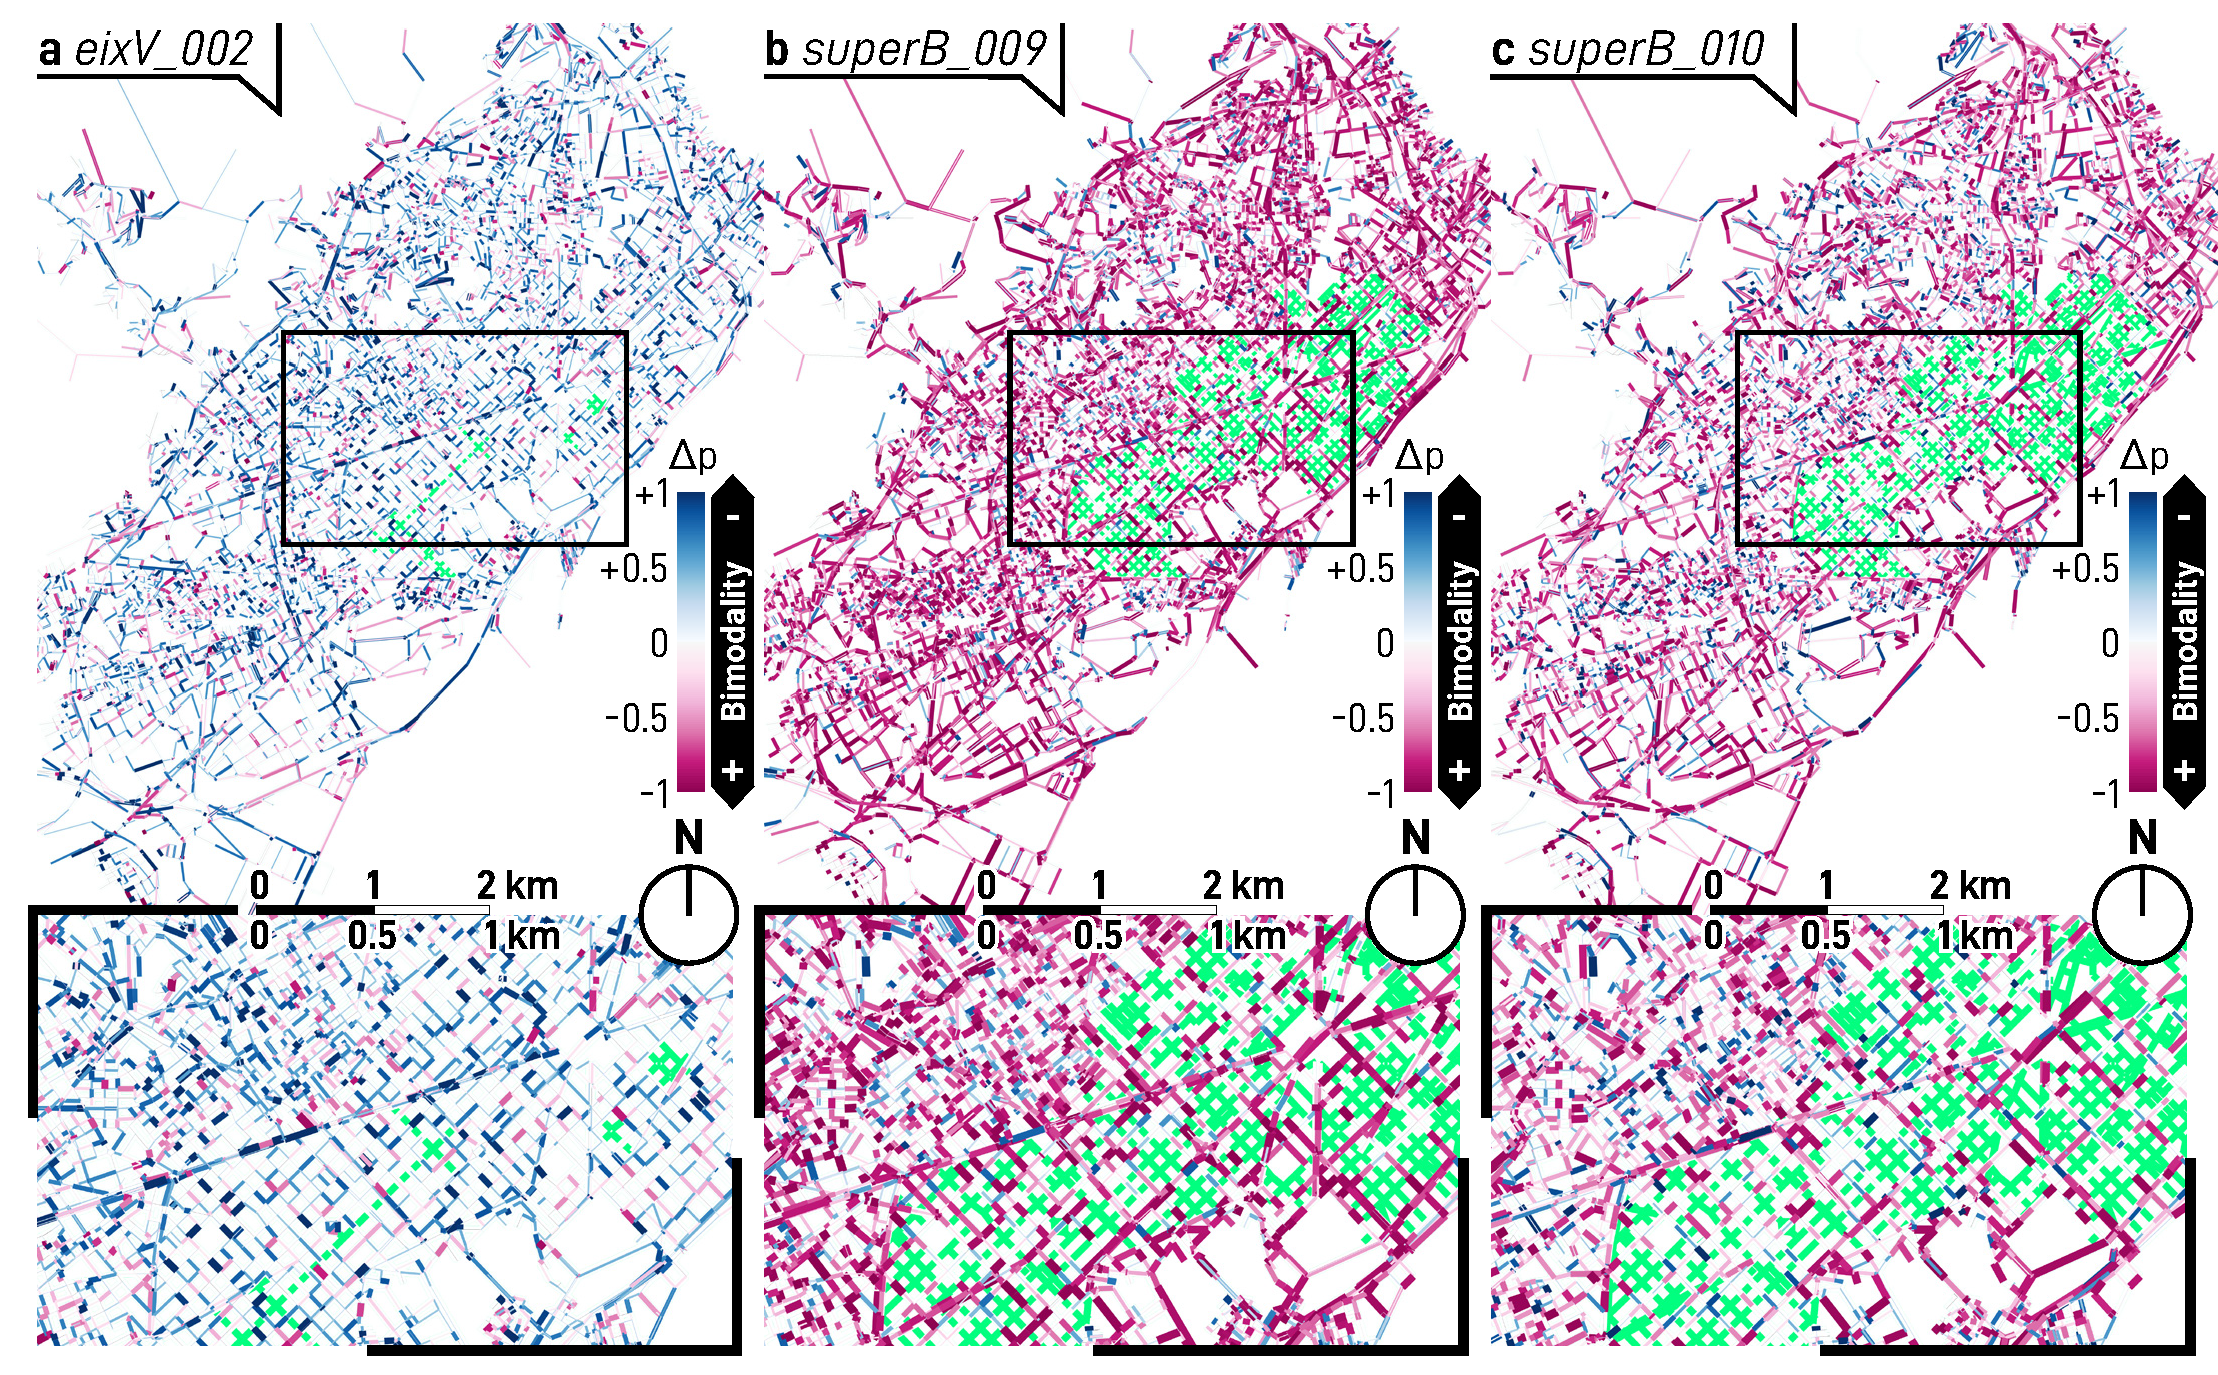
\includegraphics[width=1\textwidth]{LCBM_fig10.jpg}
    % \captionsetup{format=plain, justification=centering} % Center the caption
    \caption{Variation of the p-value per edge from Hartigan's Dip test for bimodality applied to travel times of selected scenarios compared to the baseline. A lower p-value indicates statistical significance for bimodality (e.g. scenario \emph{eixV\_002} reduces bimodality at the street level). The rectangles below each subfigure display a zoom of the central part of the city of Barcelona. Roadways closed to traffic are illustrated in green. Scenario \emph{eixV\_002} (\textbf{a}) exhibits smaller evidence for a bimodal distribution of travel times across the city (streets illustrated in blue). Scenarios \emph{superB\_009} (\textbf{b}) and \emph{superB\_010} (\textbf{c}) show a similar closure strategy, which in general, results in an increase in the evidence for bimodality across the city (streets illustrated in magenta). However, in b this increase is greater than in c. (See \cref{fig:LCBM_fig_map_03} for all scenarios).}
   \label{fig:LCBM_fig10}
\end{figure}

A further example of non-linear effects is the impossibility to link the volume of vehicles or the space available for traffic (i.e. the overall length of street sections, or the number of lanes of the closed streets) directly to the resulting level of congestion. The simplest and straightforward assumption would be that more vehicles circulating or less space available for traffic would lead to higher levels of congestion. However, this is not the case. Consequently, a moderate closing of streets following the creation of pedestrian-friendly green axes as implemented in the \emph{eixV\_002} scenario achieves the best performance (see \cref{fig:LCBM_fig11}). This means that reducing 0.41\%  of space for vehicles results in a lower level of congestion as compared to the \emph{baseline}. However, higher reductions in the space allocated to vehicles do not necessarily translate to lower levels of congestion and better environmental effects. This is evidence of the importance of non-linear effects in the simulated urban system, which are not always obvious and intuitive, but can be used to the benefit of a city.

\begin{figure}[htbp!]
    \centering
    \includegraphics[width=1\textwidth]{LCBM_fig11.jpg}
    % \captionsetup{format=plain, justification=centering} % Center the caption
    \caption{Percentage change in median time loss of selected scenarios compared to the baseline. The rectangles below each subfigure display a zoom of the central part of the city of Barcelona. Roadways closed to traffic are illustrated in green. Scenario \emph{eixV\_002} (\textbf{a}) exhibits a decrease of time loss mostly localised in two areas of the city (streets illustrated in blue) not directly adjacent to the few closed streets. Scenario \emph{superB\_009} (\textbf{b}) shows a reduction of time loss on main roads (illustrated in blue), while it increases on secondary roads (illustrated in red). Scenario \emph{superB\_010} (\textbf{c}), with a similar closure strategy to \emph{superB\_009}, exhibits a general increase in time loss across the city (illustrated in red). (See \cref{fig:LCBM_fig_map_04} for all scenarios).}
   \label{fig:LCBM_fig11}
\end{figure}

\subsection{Policy-making}
\label{subsec:LCBM_4.4_policy}

Barcelona currently envisions the Superblocks approach as an entirely new urban model \citep{AjuntamentdeBarcelona2021c} to adaptively transform the city \citep{Field2014} such that it can successfully contribute to countering climate change. This plan has not only attracted much attention in the media all over the world, but it has also become a battlefield in local politics. Therefore, the city government has put in place effective strategies for participation and engagement, to eventually gain public support for their plans. The implementation and path to success have not been straightforward, however, not only due to technical aspects. The debate also concerns issues of government authority, capitalizing on political credit, and controversies on the legitimacy of defining a determined future vision for the city, based on the respective economic and political agendas \citep{Zografos2020}.

The City of Barcelona has used citizen participation extensively to address discrepancies regarding the vision of the city and the initial criticism of excessive top-down planning and lack of transparency. Indeed, participation can improve overall results \citep{Washburn2013}, empower citizens \citep{Speer2001}, and create a common identity \citep{Campbell2000}. Hence, implementation plans were tailored to each neighbourhood and agreed upon as a result of a protocol and a road map for organizing the participation of stakeholders through joint commissions and regular meetings \citep{AjuntamentdeBarcelona2020implementingSuperblocks}. The initial Superblocks plan has since transitioned to the development of green axes (see differences between the alternatives \emph{superB\_***} and \emph{eixV\_***}) \citep{AjuntamentdeBarcelona2021SUPERBLOCKBCN}, but the effectiveness of this approach to address the societal and environmental challenges of the city has been questioned \citep{Sune2022,RuedaPalenzuela2022}.

In the participatory process mentioned above, computer simulations have been used to elaborate strategic plans. Forecasting the effects of the proposed interventions on traffic is part of the documentation to demonstrate the feasibility of the plan to the citizens \citep{AjuntamentdeBarcelona2019c,AjuntamentdeBarcelona2019b,AjuntamentdeBarcelona2013,AjuntamentdeBarcelona2018a,AjuntamentdeBarcelona2019a}. However, presenting simulations without any possibility of interacting with them may be perceived as an external and technocratic approach hindering true participation \citep{Pateman1970,Arnstein1969,ArgotaSanchez-Vaquerizo2018}. Additionally, this may be insufficient to engage citizens in the process or to inform their opinions \citep{Manzo2013}. The latest stage of scientific simulation and visualization techniques may help to overcome these issues.

In fact, the acceptance of new paradigms depends on psychosocial cognitive processes, in particular the interaction of the individual with their environment \citep{Marcheschi2022}. These interactions can promote self-exploration and collective intelligence \citep{Pan2016}, which can further improve proposed plans based on local knowledge, preferences, and values, which are often hard to grasp and encode \citep{Helbing2021}.

Overall, simulations within participatory processes should not be limited solely to legitimizing chosen frameworks and decisions. Beyond prediction, computer simulations of cities can play a pro-active, performative, and generative role in envisioning new policies through the engaged participation of citizens.

\subsection{Societal impacts}
\label{subsec:LCBM_4.5_societal_impact}

As part of the objectives of the Paris Agreement and the leadership within the C40 group, the City of Barcelona has committed itself to cutting down its CO\textsubscript{2} emissions by 45\% by 2030. Thereby it aims to reduce the effects of pollution, heat islands, and climate change on people and the environment, which is expected to be related to impacts on health and quality of life, water availability, extreme weather, temperature rise, landscape transformation, etc. \citep{AjuntamentdeBarcelona2018}. To reach this objective, the use of private motor vehicles is expected to be reduced by 20\%, local production of sustainable energy to be increased, and the energetic performance of buildings to be improved \citep{AjuntamentdeBarcelona2020a}. The effects of other air pollutants and Greenhouse Gases (GHG) on the environment and health have also been studied in detail \citep{Benavides2021,Requia2018}. Interventions on transportation have a direct impact on air quality and health, given that this source of pollution accounts for about 26\% of GHG \citep{AgenciaLocaldEnergiadeBarcelona2022}.

As shown in our computer simulations, interventions solely based on closing a few streets to motor vehicles can result in an up to 8\% reduction of emissions. Although this is insufficient to reach the ambitious environmental goals alone, the effect is still remarkable, and it exceeds the expected environmental benefits reached by all the other scenarios studied. This highlights the opportunities created by to systematically exploring non-linear, counterintuitive effects. In combination with other changes such as low emissions zones, modal share, and fleet composition through electrification, hydrogen-powered cars, and other carbon-neutral fuels, the ambitious environmental goals can be reached.

In previous studies, the environmental, health, and economic impact of the original plan of 503 Superblocks, which had initially been envisioned \citep{Rueda2018}, was estimated to cause a reduction of 24\% in NO\textsubscript{2} levels, prevent about 667 premature deaths per year, increase the life expectancy by almost 200 days, and have an economic impact of 1.7 billion Euros \citep{Mueller2020}. This quantitative health impact assessment assumes a drop of 19\% in the use of private vehicles. However, as it turns out this is not the only way to improve sustainability and health. Thus, it would be highly relevant to translate the counterintuitive complexity effects on routes, demand, emissions, and noise  into people’s health and quality of life \citep{Nagurney2000,Wang2017}. This could be accomplished by using concentration-response functions \citep{Atkinson2018} in connection to spatial factors such as population density, land use, or topography (see \cref{fig:LCBM_fig12}). Likewise, this complexity-based approach could be applied to other environmental, and health-related factors, such as physical activity, green areas, and heat \citep{Mueller2020,Woodcock2011,Gascon2016,Guo2014}.

Recently, apart from environmental and health impacts, one of the main approaches to shaping environmental policies promoted by the Sustainable Development Goals is to tax pollutant emissions in order to account for such externalities \citep{Ghazouani2020}. In the most beneficial identified scenario (i.e. \emph{eixV\_002}) the estimated savings in carbon tax \citep{Sendeco2} and fuel consumption, based on average costs for 2022, are around 10 and 80 Million Euros, respectively. Overall, this is approximately equivalent to 40\% of Barcelona’s budget for urban transformation, or to 20\% of resources allocated to social services \citep{AjuntamentdeBarcelona2021b}, i.e. quite significant.

\begin{figure}[htbp!]
    \centering
    \includegraphics[width=1\textwidth]{LCBM_fig12.jpg}
    % \captionsetup{format=plain, justification=centering} % Center the caption
    \caption{Percentage change of median CO\textsubscript{2} emissions per edge in selected scenarios compared to the baseline. The rectangles below each subfigure display a zoom of the central part of the city of Barcelona. Roadways closed to traffic are illustrated in green. Scenario \emph{eixV\_002} (\textbf{a}) exhibits a decrease of daily mostly localised in two areas of the city (streets illustrated in purple) not directly adjacent to the few closed streets. Scenario \emph{superB\_009} (\textbf{b}) shows a reduction of CO\textsubscript{2} emissions on main roads across the city (illustrated in purple), while these emissions increase on secondary roads (illustrated in orange). Scenario \emph{superB\_010} (\textbf{c}), with a similar closure strategy to \emph{superB\_009}, exhibits only an increase of CO\textsubscript{2} emissions localised in some areas of the city (illustrated in red). (See \cref{fig:LCBM_fig_map_05} for all scenarios).}
   \label{fig:LCBM_fig12}
\end{figure}

\section{Outlook and Limitations}
\label{sec:LCBM_5_outlook_limitations}

This study presents a simulation approach based on empirical data. While it uses state-of-the-art microsimulation techniques, it is important to point out limitations in its realism, e.g. related to the need of teleporting or inferring people’s routing behaviour (see also Argota Sánchez-Vaquerizo, 2021). This implies uncertainties regarding the predictive power. Nevertheless, while the resulting quantities will certainly not be exact, it is still expected that simulations like these can determine trends and some relevant features. For instance, bimodal effects are found in the baseline scenario, but can be removed by particular policy interventions that close down certain roads to motor vehicle traffic. These comparative analyses appear to be meaningful with regard to what scenarios have what characteristics, and how they perform relative to each other. 

This research is also interested in detecting existing counterintuitive effects such as improvements in traffic flows and environmental effects by closing down particular street sections. However, our paper does not try to identify Braess or Daganzo paradoxes configurations analytically or systematically \citep{Bagloee2019,Burov2021,Akamatsu2003}. Therefore, there might exist further locations where street closures would cause overall benefits. An area of future research would, consequently, be the analysis of networks from the combined perspective of structure and dynamics at different scales (in this case, temporal trends in traffic), to identify the underlying mechanisms leading to these effects. Such mechanisms may include motifs, fluctuations, and diffusion patterns \citep{Battiston2020,Arnaudon2020}. Additional non-linear effects detected between efficiency and environmental metrics should be further explored to understand when and why overall faster traffic can imply lower emissions and vice versa.

Compared to the traffic volumes which were robustly reproduced by microsimulations based on real data [74] \citep{ArgotaSanchez-Vaquerizo2021}, the realism of the total emissions data generated by the PHEMlight model is harder to assess. Studies trying to estimate the real total emissions produced by transportation in the city of Barcelona [140], [154] \citep{AgenciaLocaldEnergiadeBarcelona2022,Polo2021} are divergent, and the methodologies used are not always fully disclosed [155] \citep{Cerrillo2020}. However, the order of magnitude of the transportation-related emissions in the simulated area seems to match annual estimations [140], [155]. In the future, current microscopic traffic simulations including an emission model may be further expanded by coupling the results with multi-scale air quality and atmospheric models, combining street-scale dispersion models \citep{Holmes2006,Vardoulakis2003} with city-scale mesoscale models (e.g. Eulerian Chemical Transport Models (CTMs)) on the city scale \citep{Rodriguez-Rey2022,Brandt2003,Benavides2019,Borge2014}. Eventually, the air quality results could be compared with metrics from existing measurement stations, despite their sparsity [161] \citep{Kumar2015}. Overall, this could further improve the assessment of the health impacts of pollution.

Our study focuses on determining the complexity-related effects of varying the supply side of land transportation in cities (i.e. road infrastructure). Hence, there are additional aspects of traffic modelling and policy-making, which could be investigated in the future, such as changes in the demand or vehicle fleet composition, traffic light control, city logistics, or use of public transportation and modal share. Potential further research on causes and effects may be complemented by the use of deep learning approaches \citep{Mirzahossein2022,Zargari2022}. Already, however, the current results suggest significant expected positive effects of certain policy interventions, which can be used to make more out of the limited resources in cities (energy, space, time, etc.). In the future, it will remain interesting and relevant to look for further non-linear, perhaps counterintuitive, positive effects of various kinds and origins, which may be applied to reach a more desirable behaviour of traffic systems than what conventional changes may achieve. Among them, minimally invasive approaches appear particularly appealing.

\section{Conclusions}

This paper used microsimulations of traffic spanning 24 hours, performed for the core of the Metropolitan Area of Barcelona (2506.03 km of roads), calibrated with real cell phone data, and validated with real traffic counts. Accordingly, a quite realistic “digital twin”  was applied to test and assess different “what-if scenarios” regarding positive street closures for motor vehicle traffic. The scenarios were evaluated using efficiency-oriented and environmental metrics. By doing this, it was possible to identify at least one scenario where, after restricting motor vehicle circulation in a small part of the urban grid (0.38\% of the network length), a drop of 8\% was observed in the main pollutants while traffic conditions improved (14\% of saving time in trips) and the travel demand remained approximately the same (±2.5 \%). The direct economic impact of these savings could be equivalent to up to 40\% of the budget currently available for social services in the City of Barcelona. This is reached by counterintuitive complexity, as they are similar to those known from Braess and Daganzo paradoxes. Concretely, closing down certain roads may improve traffic performance. Hence, less can be more, if roads are closed in a smart way. This opens up important opportunities for  decision- and policy-making, using scenario analyses to promote beneficial outcomes. Therefore, the identification of counterintuitive positive effects of urban policy-making can be part of city co-creation processes, where citizens can actively explore the complexity of political, societal, health and environmental interactions through computer simulations to highlight diverse and novel sets of implications. Hence, we can summarize:
\begin{itemize}
    \item individual optimization (e.g. selfish route choice) can have undesirable outcomes compared to the system optimum;
    \item the Price of Anarchy measures the deviation from the optimal system performance;
    \item Braess and Daganzo paradoxes exemplify that more roads can sometimes increase expected travel times;
    \item while the conventional approach to overcome the Price of Anarchy problem is to control route choice, e.g. by means of road pricing schemes, alternatively, as shown in this paper, closing down selected roads for traffic smartly, may often be simpler, cheaper, and more effective to achieve traffic-related and environmental benefits.
\end{itemize}
While it was shown that the currently considered interventions may not be enough to reach all environmental and societal goals envisioned by present policies, when the vehicle fleet is not changed as well, the smart use of computational approaches to identify and reach systemic effects is promising. It may also provide new motivations for policies aiming to reach Sustainable Development Goals: if done smartly, reducing space for cars can lessen traffic congestion and pollution at the same time. In sum, novel, simulation-based, interactive approaches can contribute positively to the planning and design of our built environment, engaging the participation of stakeholders, while fostering sustainable cities. 

% \section{Additional Information}

% \subsection{CRediT authorship contribution statement}
% Javier Argota Sánchez-Vaquerizo: Conceptualization, Methodology, Software, Validation, Formal analysis, Investigation, Resources, Data Curation, Writing-Original Draft, Writing-Review \& Editing, Visualization. Dirk Helbing: Conceptualization, Supervision, Writing-Reviewing and Editing, Funding acquisition. 

% \subsection{Declaration of competing interest}
% The authors declare that they have no known competing financial interests or personal relationships that could have appeared to influence the work reported in this paper. 

% \subsection{Acknowledgements}
\section{Acknowledgements}
The authors acknowledge financial support from the European Research Council (ERC) under the European Union’s Horizon 2020 research and innovation program for the project Co-Evolving City Life (CoCi), grant number 833168. JASV wants to thank Carina I. Hausladen, Vaiva Vasiliauskaite, Sachit Mahajan, and Damian Dailisan for their help in reviewing the manuscript and the statistical methods, and Generalitat de Catalunya for providing the mobility raw data from cell phone records. Finally, the authors acknowledge using map data from OpenStreetMap contributors, and available from https://www.openstreetmap.org (accessed on 25 March 2021).



